\chapter{Doing experiments}
\section{(Initialization) A typical experimental procedure}
When doing \hl{``experiments''} using molecular dynamics we use a procedure \hl{akin to/mimicing} that used by \hl{actual} experiments. Since the duration of the experiments we are realistically able to simulate on are of the order $10^{-9}$ s / nanoseconds or below, we have to be smart when initializing the system, to avoid having to simulate for a long time to get to the state we want to study. This means that we should start out with the system in a configuration/state as close to the one we want to study as possible. The problem with this when simulating \hl{silica/glass} is that the silica structure formed when rapidly cooling molten silica doesn't have any long-range ordering. Silica in the glass form has an amorph structure, which doesn't have any long-range ordering, but has short-range ordering ``well beyond the Si-O bond length''. This structure is hard to set up with an algorithm.
%
% \orangebox{}{
%     \begin{itemize}
%         \item Remove drift!
%         \item Something smart about why the small timescales doesn't matter that much, since the length scales are equally small?
%         \item Short/long-range order
%         \item Glass transition temperature
%     \end{itemize}
%     \begin{quote}
%         ``
%         When molten silicon dioxide SiO2 is rapidly cooled, it does not crystallize but solidifies as a glass. The geometry of the silicon and oxygen centers in glass is similar to that in quartz and most other crystalline forms of the same composition, i.e., silicon is surrounded by a regular tetrahedra of oxygen centers. The difference between the glass and the crystalline forms arise from the connectivity of these tetrahedral units. Although there is no long range periodicity in the glassy network there remains significant ordering at length scales well beyond the SiO bond length. One example of this ordering is found in the preference of the network to form rings of 6-tetrahedra.[18]
%         
%         The glass transition temperature of pure SiO2 is about 1475 K.
%         ''
%         
%         \url{http://en.wikipedia.org/wiki/Silicon_dioxide#Fused_quartz}
%     \end{quote}
% }

To generate silica in the glass form we first create a perfect silica crystal in the crystalline form $\upbeta$-cristobalite, as see in figure \cref{fig:cristobalite} \todo{Why?}, and give the atoms a random uniformly distributed velocities with mean $\mu = 0$ and standard deviation $\sigma = \sqrt{T}$, where $T$ is the wanted temperature \hl{in MD units}. The crystal consists of corner-bonded SiO$_4$ tetrahedra, and in the perfect crystallic form all silicon atoms are bound to four oxygen atoms, and all oxygen atoms to two silicon atoms.
%
\begin{figure}[htpb]%
    \centering%
    \begin{subfigure}[c]{0.25\textwidth}%
%         \begin{minipage}[c]{\textwidth}%
        \includesvg[width=\textwidth, svgpath=./images/beta_cristobalite/]{beta_cristobalite_x01}%
%         \end{minipage}%
%         \caption{\cite{wikiCristobalite01}}%
        \caption{}%
        \label{fig:cristobalite01}%
    \end{subfigure}%
    \hspace{0.07\textwidth}%
    \begin{subfigure}[c]{0.45\textwidth}%
%         \begin{minipage}[c]{\textwidth}%
        \includesvg[width=\textwidth, svgpath=./images/beta_cristobalite/]{beta_cristobalite_xyz01}%
%         \end{minipage}%
%         \caption{\cite{wikiCristobalite02}}%
    \caption{}%
    \label{fig:cristobalite02}%
    \end{subfigure}%
    \caption{%
        Illustrations of the $\upbeta$-cristobalite structure, from two different views. Images from Wikipedia Commons, released to the public domain\cite{wikiCristobalite01,wikiCristobalite02}.%
        \label{fig:cristobalite}%
    }%
\end{figure}%
%
\begin{figure}[htpb]%
    \centering%
    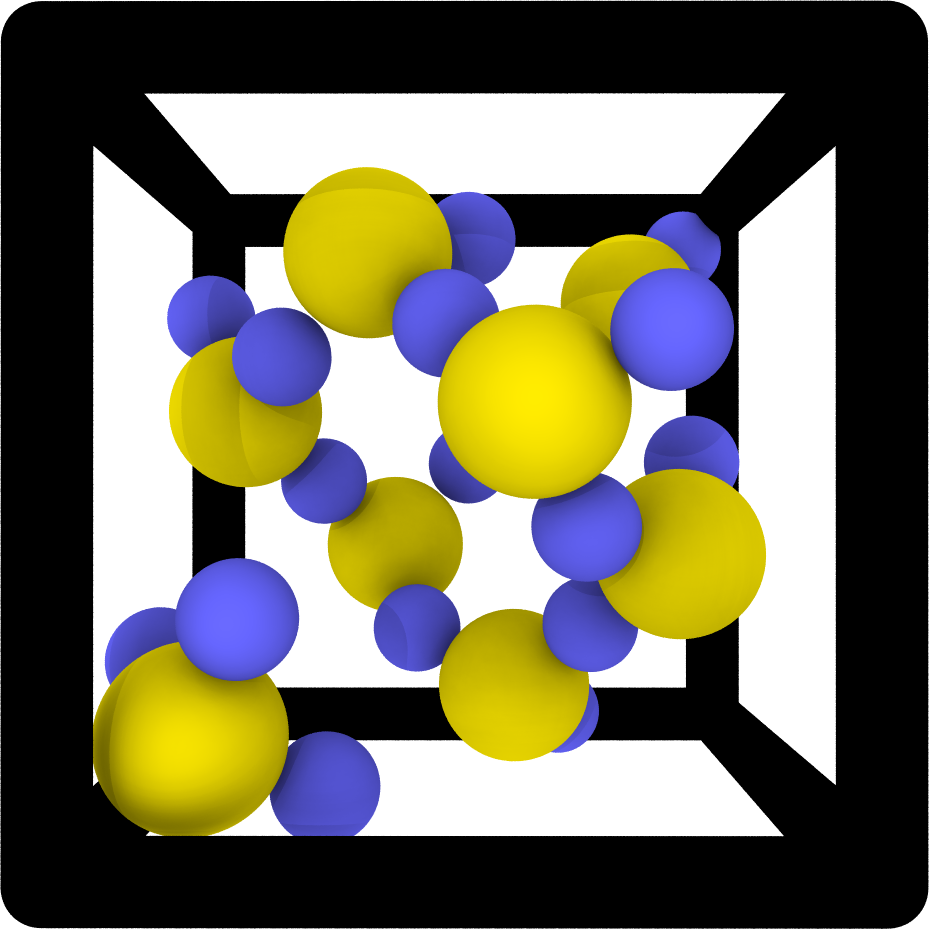
\includegraphics[width=0.6\textwidth]{images/beta_cristobalite/unit_cell03_cropped.png}%
    \caption{
        \hl{FINISH CAPTION}%
    }%
    \label{fig:beta_cristobalite-unit_cell}%
\end{figure}%

We then heat the system to 4500 K in steps of 700 K to melt the silica crystal. We alternate between using a thermostat to adjust the temperature and simulating with the thermostat off to let the system thermalize. The number of timesteps we used for the thermostat period is around 2 500, and for the thermalization period around 10 000. We then cool the system by doing the previous procedure in reverse.

We now have a thermalized and \hl{(hopefully)} realistic silica crystal at near room temperature. From this crystal we cut out the fracture, passivate using one of the passivation methods, and fill the fracture with water molecules, \hl{and use steepest descent}. After filling the fracture with water we need to thermalize the system again, since the energy (and thereby the temperature) changes when we remove and insert atoms.

We are now ready to do measurements.
%
\begin{figure}[htpb]%
    \centering%
    \begin{subfigure}[c]{0.45\textwidth}%
%         \begin{minipage}[c]{\textwidth}%
        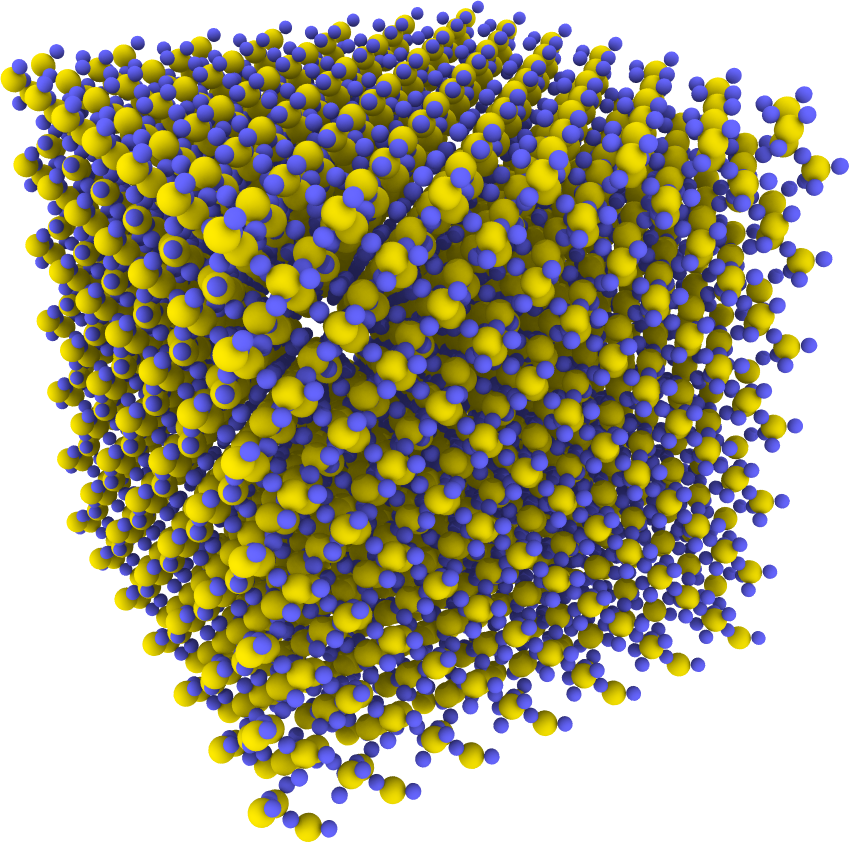
\includegraphics[width=\textwidth]{images/melt_glass/perfect_crystal02_cropped}%
%         \end{minipage}%
%         \caption{\cite{wikiCristobalite01}}%
        \caption{}%
%         \label{fig:cristobalite01}%
    \end{subfigure}%
    \hspace{0.07\textwidth}%
    \begin{subfigure}[c]{0.45\textwidth}%
%         \begin{minipage}[c]{\textwidth}%
        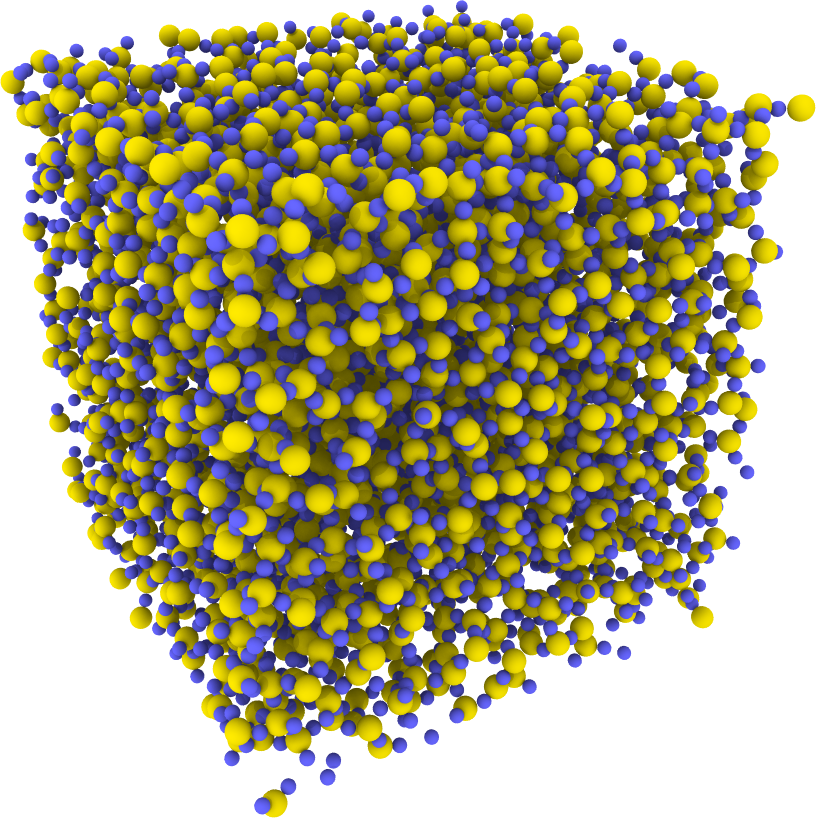
\includegraphics[width=\textwidth]{images/melt_glass/melted02_cropped}%
%         \end{minipage}%
%         \caption{\cite{wikiCristobalite02}}%
        \caption{}%+
%         \label{fig:cristobalite02}%
    \end{subfigure}%
    \caption{%
        Fig%
        \label{fig:melted_glass}%
    }%
\end{figure}%

\section{Passivation}
In most silicates the silicon atoms have tetrahedral coordination, with four oxygen atoms surronding each silicon atom. When we remove silica- and oxygen-atoms to create a fracture, we don't take this into consideration. This means that we get dangling unsaturated bonds in the system, located near the surface of the pore. To rectify this we use a method called passivation, where we saturate \hl{and passivate} the dangling bonds by inserting new atoms. 

\subsection{Water chemistry}
Since we are going to inject water into the pore later on, we want to use the constituents of water to passivate the system. We know that water autodissociates into H$^{+}$ and OH$^{-}$ via the following reaction
\begin{align*}
    \text{H}_2\text{O} \rightleftharpoons \text{H}^{+} + \text{OH}^{-},
\end{align*}
meaning that hydrogen (H) and hydroxide (OH) will be freely available in the system after filling the pore with water. On this background we choose to passivate the system using hydrogen and hydroxide. To avoid getting an \hl{acidic or alkaline / charged?} system after the passivation procedure we should make sure to use equal parts hydrogen and hydroxide when passivating.\todo{we don't whink of this when cutting though...}

\subsection{Passivating using hydrogen and hydroxide}
After thermalizing our silica system we end up with a system consisting almost exclusively of SiO$_2$ tetrahedra\todo{source? what is the rest?}. These tetrahedra are each formed by four oxygen atoms, one in each corner, and a silicon atom in the center. Each of these tetrahedra are then bonded to four other tetrahedra, by sharing the oxygen atoms in the corners. This way each oxygen atom is bonded to two silicon atoms, and each silicon atom to four oxygen atoms, giving an average chemical \hl{formula} of SiO$_2$. 

Since we don't take \hl{chemical bonds (we have no bonds...)} into consideration when removing atoms to create a fracture, we end up with some incomplete tetrahedra, with some silicon atoms bonded to less than four oxygen atoms, and some oxygen atoms bonded to less than two silicon atoms. See \cref{fig:passivation} for an illustration of three different incomplete tetrahedra. This creates what we call dangling ends/unsaturated bonds, which we want to \hl{remove/passivate}.

% When inserting hydrogen and hydroxide we want to insert them in positions that are close to their equilibrium positions, so we don't have to do a lot of simulating to get a stabilized system after passivating. It's possible to calculate the optimal positions based on the potential and the positions of the existing atoms, but this is a complicated computation, that we can avoid, by instead realizing that the optimal positions for the oxygen atoms we insert will most likely \hl{(source?)} be close to the positions that complete the SiO$_2$ tetrahedra. These positions can be calculated, using simple geometry, from the positions of the oxygen atoms each silicon atom is bonded to.

To passivate the silicon atoms that are \hl{bonded} to less than four oxygen atoms, we see that we need to complete the incomplete SiO$_4$ tetrahedra that have been created in the system. But if we only insert oxygen atoms in the positions of the missing oxygen atoms, we end up with new dangling \hl{ends/bonds}, since the inserted oxygen atoms will only be bonded to one silicon atom. But, as we just saw, we will have hydroxide (OH) groups available in the system after filling the fracture with water. So instead of inserting oxygen atoms and creating new unsaturated bonds, we insert hydroxide groups and create saturated Si-O-H \hl{bonds}. \hl{ SiO$_n$(OH)$_{4-n}$ tetrahedra.} We put the hydrogen atom so that the Si-O-H angle is close to the angle in water molecules, 107.5 degrees. \hl{The hydrogen atoms moves very rapidly compared to the rest of the species in the system, so they will quicly find the equilibrium position.}

To passivate the oxygen atoms that are bonded to only one silicon atom, we can use the hydrogen atoms that are avilable after filling the fracture with water, turning unsaturated SiO-groups into the same saturated Si-O-H-groups as before. We here too insert the hydrogen atoms with the Si-O-H angle close to 107.5 degrees.

In total we use the following procedure to passivate a system after creating a fracture:
\begin{itemize}
    \item Remove all silicon and oxygen atoms that aren't bonded to any atoms, since they are \hl{essentially} not part of the silica \hl{crystal/matrix}.
    \item Add one hydrogen atom to all oxygen atoms bonded to only one silicon atom. The hydrogen atoms are inserted approximately $0.95\text{ \AA}$ from the oxygen atoms, with the hydrogen atom pointing away from the silicon atom, and with the Si-O-H angle close to 107.5 degrees.
    \item Add ($4-n$) hydroxide \hl{molecules/groups} to silicon atoms bonded to $(1\leq n<4)$ oxygen atoms. We assume that the most stable position for the oxygen in the hydroxide groups are close to the tetrahedral positions of the missing oxygen atoms, and insert the hydroxide groups in these positions. %
    %See \cref{fig:pass_tet01,fig:pass_tet02,fig:pass_tet03} for the three different cases. 
    The hydroxide groups are inserted approximately $1.65\text{ \AA}$ from the silicon atoms, measured from the position of the silicon atom to the oxygen atom in the hydroxide groups, with the hydrogen atom pointing away from the silicon atom, and with the Si-O-H angle close to 107.5 degrees.
\end{itemize}
The lengths used are approximate experimental lengths found in naturally occuring silanols and water (see \cite{lickiss1995synthesis} for the Si-O length in silanol, and \cite{csaszar2005equilibrium} for the O-H length in water). This procedure turns all dangling ends into \hl{stable, passive} silanol groups.
%
\begin{figure}[htpb]%
    \centering%
    \begin{subfigure}[b]{0.24\textwidth}%
        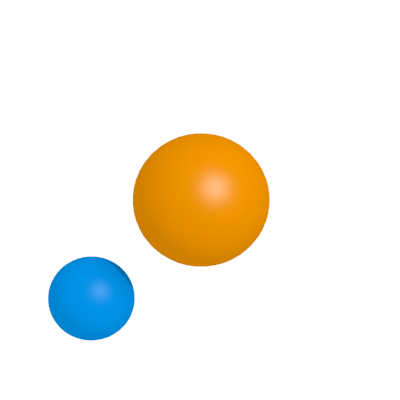
\includegraphics[width=\textwidth]{images/passivation/tetrahedra01.png}%
        \caption{}%
%         \caption{Illustration of how to divide a convex hexahedron into five tetraheda.}%
        \label{fig:pass_tet01}%
    \end{subfigure}%
%     \hspace{5mm}%
    \begin{subfigure}[b]{0.24\textwidth}%
        
\includegraphics[width=\textwidth]{images/passivation/tetrahedra02.png}%
        \caption{}%
%         \caption{A random fracture made from two periodic heightmaps.}%
        \label{fig:pass_tet02}%
    \end{subfigure}%
%     \hspace{5mm}%
    \begin{subfigure}[b]{0.24\textwidth}%
        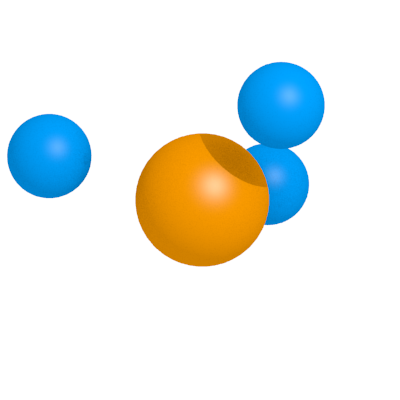
\includegraphics[width=\textwidth]{images/passivation/tetrahedra03.png}%
        \caption{}%
%         \caption{A random fracture made from two periodic heightmaps.}%
        \label{fig:pass_tet03}%
    \end{subfigure}%
%     \hspace{5mm}%
    \begin{subfigure}[b]{0.24\textwidth}%
        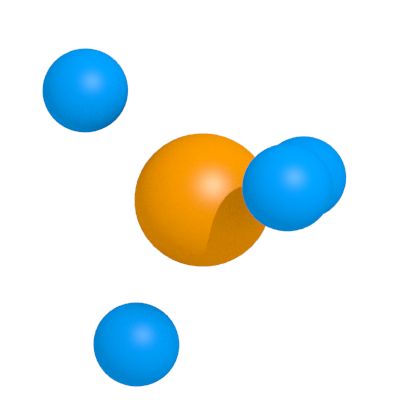
\includegraphics[width=\textwidth]{images/passivation/tetrahedra04.png}%
        \caption{}%
%         \caption{A random fracture made from two periodic heightmaps.}%
%         \label{fig:fracture_model}\caption{}%
    \end{subfigure}%
    \caption{%
        Illustration of four different incomplete silica tetrahedra, with respectively one, two, and three missing oxygen atoms. \hl{UNNECESSARY FIGURE?}
    }%
    \label{fig:passivation}%
\end{figure}%

% \begin{itemize}
%     \item Oxygen atoms with less than two silicon neighbor
%     \item Silicon atoms with less than four oxygen neighbors.
%     \item Oxygen atoms with one missing silicon neighbor.
%     \item Silicon and oxygen atoms with no neighbors.
%     \item \hl{Silicon and oxygen atoms with too many neighbors?}
% \end{itemize}

% In the passivation procedure we do some basic assumptions, based on the chemical nature of silica and water. In the thermodynamically stable form, silica should have the following properties\todo{source?}:
% \begin{itemize}
%     \item Silicon atoms should have tetrahedral coordination, with four oxygen atoms surrounding each silicon atom in a tetrahedral \hl{shape}. \todo{On average, not all silica will have this. Something about bonds? bonded to four oxygen atoms?}
%     \item Oxygen atoms should have two silicon \hl{neighbors}\todo{not all, on average}.
%     \item The Si-O distance should be in the range 1.5-1.9 pm\todo{source?} (depending on the crystalline form).
% \end{itemize}

% \hl{When removing atoms to create pores we don't care about these properties, which leads us to the following cases}


% \hl{When inserting oxygen and hydrogen we must make sure to inject neutrally, meaning twice as much hydrogen as oxygen (H$_2$O)}

% Silicon atoms with less than four oxygen atoms bound to them get ($4-n_\text{O}$) hydroxide (OH$^-$) groups attached to them, where $n_\text{O}$ is the numer of oxygen atoms bound to the silicon. Oxygen atoms with a missing silicon neighbor get a hydrogen attached. 
% % \hl{(oxygen atoms with two missing neighbors are removed)}.
% % Oxygen atoms with less than two silicon atoms get ($2-n_\text{Si}$) hydrogen atom attached, where $n_\text{Si}$ is the number of silicon atoms bound to the oxygen. 
% 
% When passivating a silicon atom with missing oxygen neighbors by \hl{simply} filling in the missing atoms to complete the SiO$_4$-tetrahedra. We then put one hydrogen atom on each new oxygen atom, to avoid dangling bonds on the inserted oxygen atoms.
% 
% When passivating a oxygen atom with a missing silicon neighbor, we put one hydrogen atom on the opposite side of the oxygen atom compared to the silicon atom.
% 
% All silicon and oxygen atoms with no neighbors we remove, since they aren't really part of the silica.

\subsection{Counting number of bonds}
Since we don't have actual bonds in molecular dynamics simulations, we don't know what the actual bonds look like. So to find the number of \hl{neighbors/bonds/bonded atoms} for each silicon and oxygen atom, we create what we call \emph{neigbor lists}, which is a list of atoms within a chosen radius, for each atom. To create these lists we use the procedure detailed in \cref{sec:neighbor_lists}. Since we only have silicon and oxygen atoms in our system, we only need to specify a maximum the Si-O-distance to find which atoms are bonded. If we choose this distance properly, we should be able find a good approximation to how many atoms each atom is bonded to.

\orangebox{
\begin{itemize}
    \item What Si-O distance did we use to find bonds? Why? 
    \item g(r) for Si-O?
    \item Implementation?
    \item Visualization of results?
    \item What to do about atoms that can't be passivated (because we have to insert passively)?
\end{itemize}
}

% \subsection{Implementation}
% To implement the passivation procedure detailed above we see that we can make an  

% \begin{itemize}
%     \item Tetrahedra
%     \item Neighbor lists -- see base\_code/passivate\_using\_tetrahedra/passivator.cpp near line 700
%     \begin{itemize}
%         \item Create list of atoms in each voxel
%         \item Create neighbor lists for each atom by looping through neighbor voxels for each atoms
%     \end{itemize}
%     \item Count number of neighbors of different types -- find number of missing neighbors, Si - 4 Oxygen, Oxygen 2 Si
%     \item Insert OH on Si with missing O neighbors, insert H on Oxygen with missing Si neighbors
%     \begin{itemize}
%         \item Insert O/H at good angles
%     \end{itemize}
%     \item Improvement: find the atoms near surface using voxels, only passivate those atoms
% \end{itemize}

\subsection{Only passivating surface atoms}
When implementing the passivation method detailed above, we soon ran into problems with silica and oxygen atoms that were bonded to too few atoms according to our rules above, while counting the number of bonds using a fixed radius. Some improvements were made by fine-tuning the radius used for each atom type, but we still often ended up passivating atoms that were inside the silica matrix, where we shouldn't have any dangling \hl{bonds/ends}. To avoid this we came up with a method to only passivate the atoms \hl{at or near} the surface of the fracture.

To do this we \hl{yet again} use the voxelation method from \ref{sec:voxelation}, but this time we use a voxel size of around $6\text{ \AA}$. We then mark all voxels with atoms in them as occupied. We now see that if we find all \emph{occupied} voxels with at least one \emph{unoccupied} neighbor voxel \hl{(using 26-neighbor connectivity)}, we should have a list of the voxels that make up the surface of the fracture, and these voxels then contain all atoms at or near the surface of the fracture. We then use this list of atoms as input to the passivation program, and only passivate atoms in that list. See \cref{fig:find_surface_atoms} for an illustration of the method that finds the voxels and atoms at the surface of the fracture.
%
\begin{figure}[htpb]%
    \centering%
    \includesvg[width=0.5\textwidth, svgpath = ./images/passivation/]{select_surface_voxels05}%
    \caption{
        Illustration of a method for finding atoms and voxels at the surface of a fracture. All gray voxels are occupied voxels (with at least one atom in them), and the dark gray voxels are the voxels with at least one unoccupied neighbor voxel. \hl{FINISH} \hl{change to v1 of illustration?} \hl{what size shoud fig be? 0.4 maybe a bit small?}
    }%
    \label{fig:find_surface_atoms}%
\end{figure}%

\subsection{Results/examples}
An example of a system after passivation can be seen in \cref{fig:passivation_example}. Here we see hydrogen and ???
%
\begin{figure}[htpb]%
    \centering%
    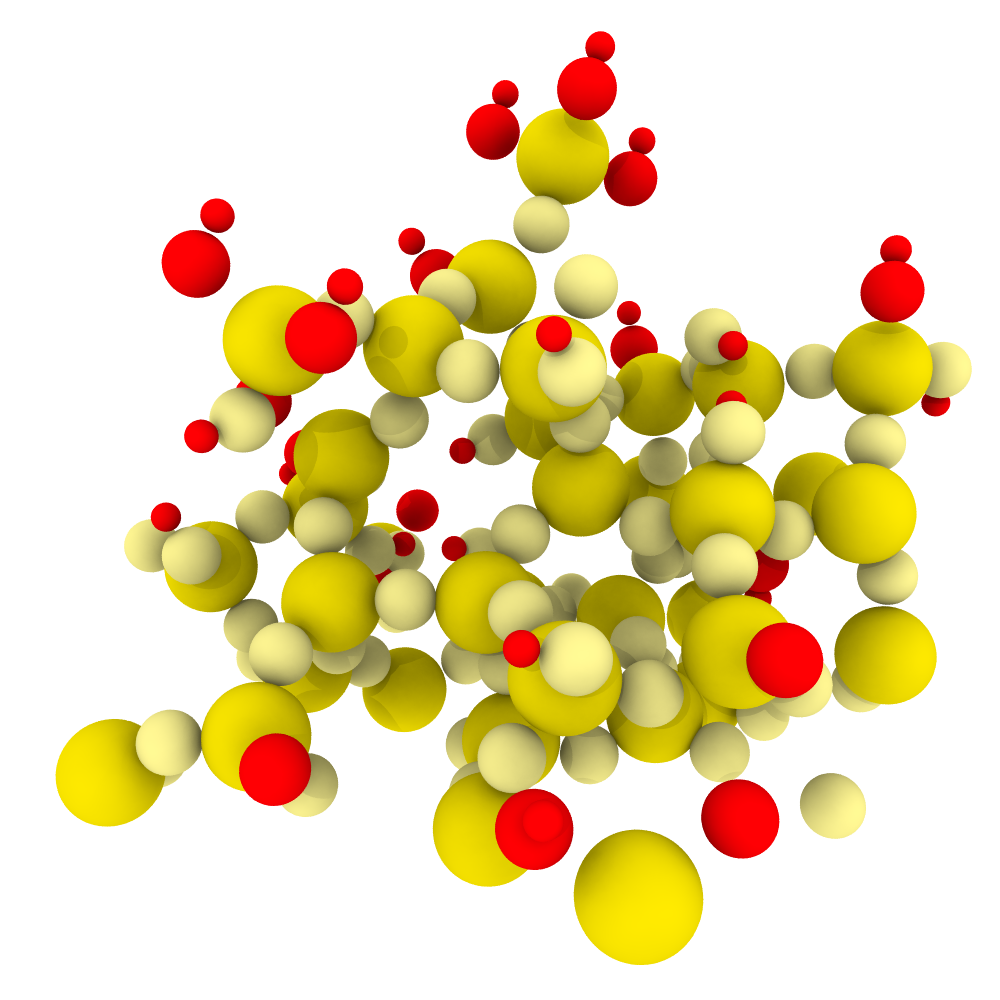
\includegraphics[width=0.7\textwidth]{images/passivation/passivation_example04.png}%
    \caption{
        Passivation example.png.\hl{FINISH CAPTION}%
    }%
    \label{fig:passivation_example}%
\end{figure}%

\FloatBarrier
\section{Injecting water}
After removing atoms to create a fracture, and passivating the system, we are now ready to inject water into the fracture. To do this we use the technique of \emph{voxelation} (see \cref{sec:voxelation}). We first divide the system into voxels, find the empty voxels, and then put one water molecule in each unoccupied voxel. The water density can then be controlled by the size of the voxels we use.\todo{Not filling all voxels}

\subsection[Finding correct voxel size/water density?]{Finding correct voxel size/\hl{water density?}}
If we want to inject water with density $\rho$% [kg/m$^3$]
, we can find the voxel size we need from the molar mass of water, $M_\text{H$_2$O} = M = 0.0180158 \text{ kg/mol}$\hl{SOURCE}. We use the molar mass and wanted density to find the ``volume'' each water atom should occupy% , the unit used in the \hl{MD integrator/program and output files}
, as follows
% \begin{align*}
%     V 
%     &= \frac{ M\text{ [kg/mol]} }{ \rho\text{ [kg/m$^3$]} } \\
%     &= \frac{
%             M\text{ [kg/mol]} \times \dfrac{1}{N_A \text{ [mol$^{-1}$]}}
%         }{
%             \rho\text{ [kg/m$^3$]} \times \left(10^{-10} \text{ [\AA/m]}\right)^3
%         } \\
%     &= \frac{M}{\rho} \times \frac{10^{-30}}{N_A} \text{ [\AA$^3$]},
% %     \times \frac{N_A \text{ [mol$^{-1}$]}}{10^{-10} \text{ [\AA/m]}} 10 \text{ [m$^3$]} \\
% \end{align*}
\begin{align*}
    V 
    = \frac{ M\text{ [kg/mol]} \times \dfrac{1}{N_A \text{ [mol$^{-1}$]}}}{ \rho\text{ [kg/m$^3$]} } 
    = \frac{M}{\rho N_A}\text{[m$^3$]}
\end{align*}
where $N_A$ is the Avogadro constant. From here we find the size we need our voxels by taking the cube root
% \begin{align*}
%     l = \left(\frac{M}{\rho} \times \frac{10^{30}}{N_A}\right)^{1/3}\text{ [\AA]}.
% \end{align*}
\begin{align*}
    l = \left(\frac{M}{\rho N_A} \right)^{1/3}\text{ m}.
\end{align*}
We then divide the system into voxels of length $l$, and put one water molecule with random orientation in the center of each empty voxel. If we for example want to insert water with $\rho = 1000\text{ kg/m}^3$, approximately the density of water in room temperature\hl{SOURCE}, we get a voxel size of
\begin{align*}
    l = \left(\frac{0.0180158 \text{ kg/mol}}{1000\text{ kg/m$^3$} \times 6.0221 \times 10^{23}\text{ mol$^{-1}$}} \right)^{1/3} = 3.1 \text{ \AA}.
\end{align*}

\subsection{Finding empty voxels}
The naive way of finding the empty voxels is to just find which voxel each silicon and oxygen atom is in, and mark those as occupied. Using this method we found that we often got some empty voxels inside the silica matrix, which meant we got single water atoms trapped inside what was supposed to be the silica matrix. 

This can be explained if we compare the voxel size of $3.1 \text{ \AA}$ in water with a density of $\rho = 1000\text{ kg/m$^3$}$, as we found above, to the typical Si-O bond length in silica. \todo{better explanation}When we take into account the amorphous structure of silica we see that it's likely that we get some small pores with room for a water atom in between some of the silica tetrahedra.

To solve this we assign a radius to each atom type\todo{which is hard, Si-O, ???}, and mark all voxels with the center of the voxel within this radius from an atom as occupied. See \cref{fig:inject_empty_voxel} for an illustration of this procedure. 
%
\begin{figure}[htpb]%
    \centering%
    \begin{subfigure}[b]{0.45\textwidth}%
        \includesvg[width=\textwidth, svgpath=./images/inject_water/]{drawing02}%
%         \caption{}%
        \caption{Marking only one voxel per atom as occupied.}%
%         \label{fig:pass_tet01}%
    \end{subfigure}%
    \hspace{0.05\textwidth}%
    \begin{subfigure}[b]{0.45\textwidth}%
        \includesvg[width=\textwidth, svgpath=./images/inject_water/]{drawing_radius02}%
%         \caption{}%
        \caption{Marking all voxels within radius from atom as occupied.}%
%         \label{fig:pass_tet02}%
    \end{subfigure}%
    \caption[
        To find voxels we can put water molecules in we can either \textbf{a)} mark the voxel each atom belongs in as occupied, or \textbf{b)} mark all voxels within a radius from each atom as occupied. We can assign a different radius to each atom. We have illustrated using part of a silica tetrahedra, with one silicon atom (the large blue dot) and two oxygen atoms (the smaller red dot). The center of each voxel is marked by a dot 
    ]{%
        To find voxels we can put water molecules in we can either \textbf{a)} mark the voxel each atom belongs in as occupied, or \textbf{b)} mark all voxels within a radius from each atom as occupied. We can assign a different radius to each atom. We have illustrated using part of a silica tetrahedra, with one silicon atom (
\includegraphics[scale=0.8]{./images/inject_water/silicon.pdf}) and two oxygen atoms (\raisebox{0.3ex}{
\includegraphics[scale=0.8]{./images/inject_water/oxygen.pdf}}). The center of each voxel is marked by a dot. \hl{Maybe change to v01 of images?} \hl{This voxel size is pretty tiny...}
    }%
    \label{fig:inject_empty_voxel}%
\end{figure}%

A different solution to the problem of tiny pores inside the silica matrix is to \hl{just} remove all small clusters of voxels (where a ``small cluster of voxels'' would need to be defined)\hl{, which sometimes can be a better solution, since we introduce new lone voxels when making radius? Maybe implement both methods, a small radius and remove small clusters?}.

\orangebox{
\begin{itemize}
    \item Remove tiny pores?
    \item Mark all voxels within distance from other atoms as occupied
    \item Fill other voxels with H2O with random O-H orientation, but correct angle
    \item Improvement: Use one voxel size in the beginning (to avoid one-voxel pores), and then use a smaller voxel size when injecting water
\end{itemize}
}

